\documentclass[uplatex,dvipdfmx,a4paper,11pt]{jsarticle}

\usepackage{amsmath,amsthm,amssymb}
\usepackage[dvipdfmx]{graphicx}
\usepackage{bm}
\usepackage{ascmac}
%
\usepackage{multirow}
\usepackage{wrapfig}

% \pagestyle{empty}
% \usepackage[truedimen,margin=20truemm]{geometry}

% \renewcommand{\baselinestretch}{0.9} % 全体の行間調整
% \renewcommand{\figurename}{Fig.}
% \renewcommand{\tablename}{Tab.}
% \usepackage{setspace}
%
\pagestyle{empty}
% 高さの設定
\setlength{\textheight}{\paperheight}   % ひとまず紙面を本文領域に
\setlength{\topmargin}{-5.4truemm}      % 上の余白を20mm(=1inch-5.4mm)に
\addtolength{\topmargin}{-\headheight}  % 
\addtolength{\topmargin}{-\headsep}     % ヘッダの分だけ本文領域を移動させる
\addtolength{\textheight}{-40truemm}    % 下の余白も20mmに%% 幅の設定
\setlength{\textwidth}{\paperwidth}     % ひとまず紙面を本文領域に
\setlength{\oddsidemargin}{-5.4truemm}  % 左の余白を20mm(=1inch-5.4mm)に
\setlength{\evensidemargin}{-5.4truemm} % 
\addtolength{\textwidth}{-40truemm}     % 右の余白も20mmに

%
\abovecaptionskip=-1pt
%\belowcaptionskip=-1pt
%
\renewcommand{\baselinestretch}{0.9} % 全体の行間調整
\renewcommand{\figurename}{Fig.}
\renewcommand{\tablename}{Tab.}
%
\makeatletter 
\def\section{\@startsection {section}{1}{\z@}{1.5 ex plus 2ex minus -.2ex}{0.5 ex plus .2ex}{\large\bf}}
\def\subsection{\@startsection{subsection}{2}{\z@}{0.2\Cvs \@plus.5\Cdp \@minus.2\Cdp}{0.1\Cvs \@plus.3\Cdp}{\reset@font\normalsize\bfseries}}
\makeatother 
%
\graphicspath{{../../figures//}}
%
\begin{document}

%%%%%%
% はじめに
%%%%%%
\begin{center}
{\Large \textgt{22. ランダム構造を有するネットワークポリマーの緩和挙動}}
\end{center}

\begin{flushright}
東亞合成 佐々木裕

Tel: 052-611-9923, e-mail: hiroshi\_sasaki$@$mail.toagosei.co.jp
\end{flushright}

\vspace{0.5\baselineskip}
\section{はじめに}

近年、ソフトマターの階層的な構造設計の考え方が深化し、力学特性に優れたネットワークポリマーの材料設計にも応用されている。

旧知の材料であるゴムの大きな破壊靭性の由来については、その破壊エネルギーがヒステリシスロスと良い相関を示すことが報告されており~\cite{payne1}、クラック先端でのエネルギー散逸により亀裂進展が抑制されるという Andrews モデルが提案されている\cite{andrews}。
また、そのヒステリシスロスの発現機構として、 Payne は、1) 粘弾性に基づくもの、2) 結晶化に由来するもの、3) 添加したフィラーに起因したものの3つに大きく分類している~\cite{payne2}。
ヒステリシスの原因として、フィラー由来、あるいは、伸張結晶化のようなメゾスケール領域の挙動に注目する場合が多く見受けられる~\cite{zhang}。
一方、ゴム系材料の破壊において時間温度換算則が大変形を伴う破壊挙動にも成立し、室温では容易に破断する SBR がガラス転移温度に近い低温での伸長では高い伸びと強度を示すことも報告されている~\cite{smith}。
この時間温度換算則については粘弾性効果に基づくものとして取り扱うべきであり、その由来をミクロな分子描像で記述できるかもしれない。

ゴム弾性の古典的なモデルである ``Affine Network Model'' からの発展形として、結節点の揺らぎに注目した``Phantom Network Model: PNM''が提案され、Flory によればメルト状態と同一なストランドのゆらぎを有するランダムネットワークにおいて PNM のふるまいを示すとされている~\cite{flory}。
我々は、この結節点のゆらぎ由来の散逸が、分子鎖描像のようなミクロなスケールでの粘弾性的な挙動のモデルとなりうるのではないかと考え、これまで検討を進めている。

以前に、ネットワーク構造の接続性をランダムへと変えることで架橋欠損のないネットワークを作成して PNM を再現できることを報告した~\cite{sasaki}。
本報告では、ランダムな接続性を有するネットワークポリマーを用いて、その力学特性と緩和挙動との関係について、MD シミュレーションにより検討した結果について報告する。

\section{シミュレーション}
既報~\cite{sasaki}に従い、任意の分岐数$f$($f=3\sim6$)の結節点からなるランダムな接続性を有するネットワークを作成し、その平衡状態および変形(一軸伸張およびずりせん断)時の振る舞いについて、OCTA 上の COGNAC シミュレーターを用いた分子動力学シミュレーションにより評価した。

\subsection{ネットワークモデルの作成}
トポロジーモデルの「代数的連結性」を指標として以下のアルゴリズムでランダムな結合性を導入した。
% \vspace{-2mm}
\begin{enumerate}
\item
実空間での初期構造を体心立方構造の各格子点をストランドでつないだ「八本鎖モデル」として、それに対応するように任意の分岐数のトポロジーモデルを作成。
% (Fig. \ref{fig:topo})。
\item
代数的連結性を指標としてストランド交換し、結節点の結合性にランダム性を導入。
% (Fig. \ref{fig:exc})。
\item
そのトポロジーモデルに対応するように、実空間の初期構造からストランドを除去。
\end{enumerate}

\subsection{初期構造の作成}
任意のセグメント数のストランドを用いてストランドの末端間距離がホモポリマーメルトと同等になるようにユニットセル長と多重度を調整し、KG 鎖の一般的な密度 ($\rho$=0.85) となるモデルを作成した。

\subsection{MD シミュレーション}
セグメント間の非結合ポテンシャルに斥力($r_c = 2^{1/6}\sigma$)である LJ ポテンシャル $U_{LJ}(r_{ij})$、ボンドポテンシャルには FENE-LJ ポテンシャルを用いて KG 鎖とした。
なお、初期構造の緩和は Auhl 等の方法~\cite{Auhl} に従い force-capped-LJ ポテンシャルを用いて、段階的にす抜け鎖から絡み合い鎖へと遷移させた。
初期緩和終了後に、Kr\"{o}ger らの方法~\cite{Kroger} によりストランド同士の絡み合いを評価して、対応するホモポリマーメルトと同程度であることを確認した。
% また、密度の低い初期状態から NPT 計算により圧縮することで、絡み合いを極力排除した比較計算も実施した。

\section{結果と考察}

\subsection{PNMの確認}
同一のストランド長(セグメント数: 20)を有する 3, 4, 6 分岐のネットワークポリマーにおける変形速度依存性が消失するせん断変形($\dot{\gamma} \simeq 5e^{-5}$)での SS カーブ(Fig. \ref{fig:deform})より、PNM が示す弾性率 $G$~\cite{flory}に比例する形での以下の関係が示された。
\vspace{-2mm}
\begin{align*}
    &G = g \left(1-2/f\right) \nu k_BT \\ &\text{where $g \simeq$ 2}
\end{align*}
\vspace{-5mm}

ここで示された 2 程度の定数因子 $g$ については、システムサイズ依存性は小さく、ストランド長および排除体積効果の影響が見られたが、詳細は検討中である。

\subsection{ヒステリシスロスの速度依存性}

4分岐のネットワークにおいてPNM へと漸近する変形速度 ($\dot{\gamma} = 2e^{-4}$) で周期的な変形 ($\gamma = 1$) を付与した結果を Fig. \ref{fig:hyst} に示した。
複数回の変形に対しても迅速な回復を伴った力学的ヒステリシス (Hysteresis loss $\simeq$ 0.34) を示すことが確認できた。

各種の変形条件でのヒステリシスロスの振る舞いを、Fig. \ref{fig:hystloss} に示した。
高速変形では大きな値を示したが変形速度の低下に伴い減少し、$\dot{\gamma} \sim 1e^{-5}$ 程度のオーダーの時間スケールで消失するようであった。

\subsection{最長緩和時間の検討}
4分岐のネットワークの長時間緩和後の平衡構造において、ラウスモード(p=1)の自己相関関数 $C_p(t)$ から最長緩和時間 ($\tau$) について評価し、$\tau \simeq 6.5e^{4}$ を得た。

この緩和時間の長時間化はネットワーク構造に起因した架橋点の運動性の低下によるものと想定でき、長鎖のホモポリマーメルトでの絡み合いに起因したラウスモードのふるまい~\cite{rubinstein} と合致していた。
また、この値の逆数は前述のヒステリシスロスが消失する変形速度と対応するものと考えられた。
\vspace{-1mm}
\begin{figure}[hb]
\begin{minipage}{0.33\hsize}
    \begin{center}
        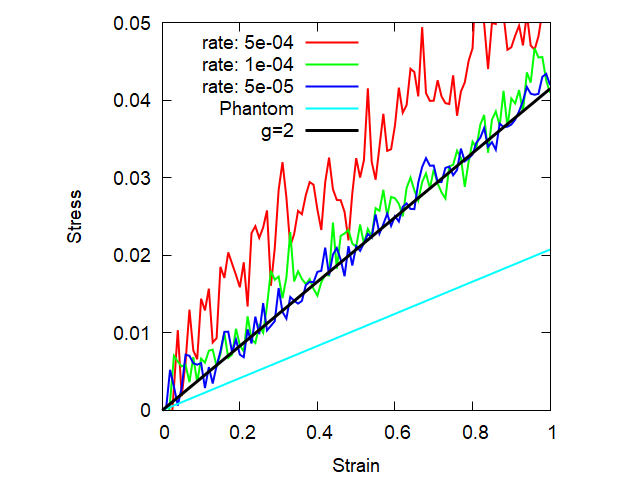
\includegraphics[width=.9\textwidth]{Shear_Random_4chain_N20_g2.png}
        \caption{Stress-Strain Curves for 4-chain NW at varied shear rate ($\dot{\gamma}: 5e^{-4} \sim 5^{e-5}$)}
        \label{fig:deform}
	\end{center}
\end{minipage}
\begin{minipage}{0.33\hsize}
	\begin{center}
        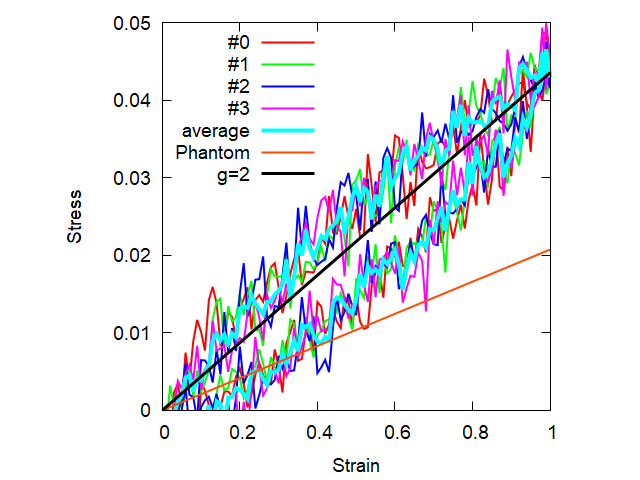
\includegraphics[width=.9\textwidth]{CyclicDeform_4chain_rate_2e-4_g2.png}
        \caption{Hysteresis Curves for 4-chain NW by Cyclic Shear ($\gamma = 1$), shear rate $\dot{\gamma} = 2e^{-4}$}
        \label{fig:hyst}
	\end{center}
\end{minipage}
\begin{minipage}{0.33\hsize}
	\begin{center}
        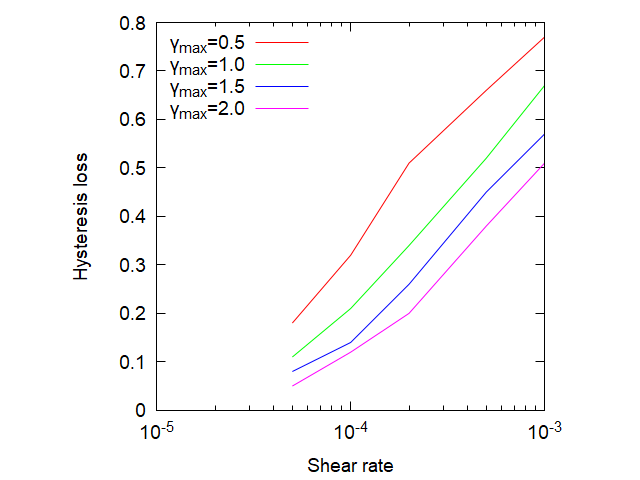
\includegraphics[width=.9\textwidth]{hyst_shear.png}
        \caption{Hysteresis losses for varied shear rates and maximum strains for 4-chain NW}
        \label{fig:hystloss}
	\end{center}
\end{minipage}
\end{figure}

\vspace{-7mm}
\begin{thebibliography}{99}
    \bibitem{payne1} K. Grosch, J.A.C. Harwood \& A.R. Payne, Nature, 212 5061 497 (1966)
    \bibitem{andrews} E. H. Andrews, Y. Fukahori, J. of Mat. Sci., 12, 1307 (1977)
    \bibitem{payne2} A. R.Payne, J. Polym. Sci. Part C, Polym. Symp., 48(48), 169 (1974)
    \bibitem{zhang} H. Zhang et al. Macromolecules 46, 900 (2013)
    \bibitem{smith} T. L. Smith, R. A. Dickie, J. of Polym. Sci. A-2: Polym. Phys., 7, 635 (1969)
    \bibitem{flory} P. J. Flory, Proc. R. Soc. London. Series A, 351, 351 (1976)
    \bibitem{sasaki} 佐々木裕, 第69回レオロジー討論会 (2021)
    \bibitem{Auhl} R. Auhl et al., J. of Chem. Phys., 119, 12718 (2003)
    \bibitem{Kroger} S. Shanbhag, M. Kr\"{o}ger, Macromol. 40 2897 (2007)
    \bibitem{rubinstein} J. T. Kalathi et al., Macromol. 47 6925 (2014)
\end{thebibliography}

\end{document}